\chapter{Introduction}
\label{sec:intro}
\lhead{\emph{Chapter 1. Introduction}}  % page header

\begin{figure}[t]
  \centering
  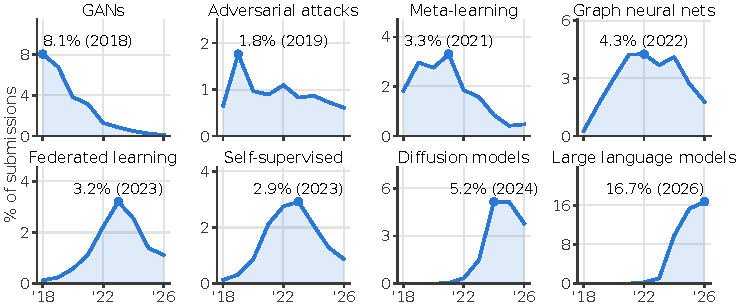
\includegraphics[width=\textwidth]{figs/fig1_waves.pdf}
  \caption[Research waves at ICLR, 2018--2026]{Research waves at ICLR: share of discovery submissions listing each author keyword, 2018--2026; dots
  mark the peak. The eight keywords were chosen for display after their curves were known. Across the 68 most
  frequent keywords, 17 peaked in 2019--2024 with shares of at most half the peak both before it and in 2026.
  Uses no acceptance data.}
  \label{fig:waves}
\end{figure}

Machine learning is often said to herd. Between 2017 and 2026, yearly submissions to the International Conference
on Learning Representations (ICLR) in our discovery corpus grew 40-fold, from 384 to 15,411. The share building on a
foundation model (FM) rose from 0.3\% to 54.4\%, and the share proposing a new architecture fell from 24.5\% to
7.5\%. Keywords rose and fell (Figure~\ref{fig:waves}): generative adversarial networks fell from 8.1\% of
submissions in 2018, and large language models reached 16.7\% in 2026. The wave is NLP's too, as its researchers
increasingly publish at ML venues \citep{jurgens2026future}. Whether science has fashions is an old question
\citep{crane1969fashion}. Critics of ML scholarship point to incentives that favour short-term success
\citep{lipton2019troubling} and to convergence on what suits the field's hardware, benchmarks and foundation models
\citep{hooker2021hardware,dehghani2021benchmark,bommasani2021opportunities}; cascade and fashion theories explain
waves by people taking their cue from others
\citep{bikhchandani1992theory,banerjee1992simple,abrahamson1991managerial}.

Is the switch to FMs not herding enough? Convergence on a shared substrate is
predicted by lock-in, by the efficient choice of a tool that works and by a bandwagon alike, so the curve cannot tell
them apart. The herding question is about behaviour: what researchers write when they enter a topic, and what the
review gate accepts. There, two routes to conformity part. \emph{Imitation} takes its reference point from what
others are doing now: what is popular, rising or recently accepted. \emph{Continuity} takes it from a record: the
team's own earlier work, or a topic that a team member already knows. Imitation makes teams alike; continuity keeps
each team near its own past. We call work that conforms by continuity \emph{anchored}.\footnote{`Anchored' names a position relative to a record, not a mechanism.
It is not the anchoring-and-adjustment heuristic \citep{tversky1974judgment}, the sense in which writing on herding
in science uses the word \citep{baddeley2015herding}.}

Read as herding, the waves make three claims: they are fashions; newcomers to a topic carry them by following
others; and review favours following. We test each claim at its site, the field, entry to a topic and the
acceptance gate, on 43,480 ICLR submissions from 2017--2026, rejected and withdrawn papers included. Hypotheses
were registered before any full-corpus label existed, outcomes stayed sealed until one frozen run, and the main tests were run again on 11,099 held-out papers: a pre-registered out-of-sample replication, not a
certified untouched holdout. Each finding carries one of three labels: \lab{replicated} (from a registered test,
supported again on held-out papers), \lab{held-out supported} (found post hoc, then supported by a
test declared before the held-out data were read) or \lab{exploratory} (discovery only, or descriptive). Tests
without a verdict are called inconclusive or uninformative (Chapter~\ref{sec:design}).

At the field level, keyword waves are real, but emergence depends on hindsight, and the durable shift, the FM
package, fits every route. At entry, researchers new to a topic propose methods more often than incumbents, while,
in the FM era, benchmark and evaluation work sits with incumbents: the opposite of the follow-on entry that herding
implies, and of our own registered prediction. At the gate, no premium for crowded topics is detectable, the branded
title's small premium lies below what the held-out test could detect, and what replicated, apart from regressing
topic edges, is tied to the team's own record.

Prior work relates ICLR acceptance to prestige, process and research area
\citep{tran2020open,ibrahim2026bias,jung2025what,wang2023what,xu2026reviewer} and describes which papers start
topics, who enters LLM research and how far researchers move from their own past work
\citep{huang2026catalyst,movva2024topics,bao2025persistence}. To our knowledge, among the works we checked, none
tests the herding account at entry and at the gate within one submission population, with registered hypotheses
re-tested on held-out papers, as \citet{ibrahim2026bias} did for a prestige gap. We contribute:
\begin{itemize}[leftmargin=*,itemsep=1pt,topsep=3pt,parsep=0pt]
\item \textbf{Entry.} A registered test of herding where imitation predicts it most sharply. Researchers entering a
topic propose methods more often (+3.7\,pp; \lab{replicated}). The surplus holds for researchers with ICLR work in
other topics and predates the FM wave, while, in the FM era, benchmark and evaluation work sits with topic
incumbents and larger teams (\lab{exploratory}).
\item \textbf{Gate.} Using every decided submission under double-blind review, rejected ones included, acceptance
goes with closeness to the team's own record among teams that have one (far jump $-$5.4\,pp, held-out $-$6.1;
\lab{held-out supported}), not detectably with the crowd.
\citet{hill2025pivot} relate pivots to publication success; we add the accept/reject decision itself.
\item \textbf{Method.} On the same papers, the number of emerging topics ranges from 8 to 29 depending on the
years the topic map is fitted on (\lab{exploratory}). Emergence is hard to judge before the fact
\citep{rotolo2015what,li2025evaluation}, and a prospective signal has been tested \citep{khanbayov2026topical};
an early-window refit is a cheap check on trend claims.
\end{itemize}

% ===============================================================================================================
